\documentclass{article}
\usepackage[utf8]{inputenc}

% Page setup
\usepackage[a4paper,landscape,margin=2cm]{geometry}
\usepackage{amsmath}

% Typography
\usepackage[scaled]{helvet}
\let\familydefault\sfdefault

\usepackage[usenames,svgnames]{xcolor}
\usepackage{tikz,pgfplots}
\usetikzlibrary{positioning,arrows,intersections,calc}

\definecolor{one}  {RGB}{142, 23,  4}
\definecolor{two}  {RGB}{ 62,111,186}
\definecolor{three}{RGB}{172,196, 75}

\begin{document}
\pagestyle{empty}
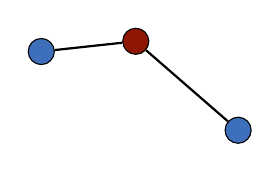
\begin{tikzpicture}[every node/.style={draw,shape=circle,fill=two}]

    \node (a) at(0,0) {};
    \node (b) at(2.5,-1) {};
    
    \node[fill=one] (d) at(1.2,0.13) {};
    
    \draw[thick] (a) -- (d);
    \draw[thick] (d) -- (b);

\end{tikzpicture}
\end{document}
